% fixture: tikz/trees
% tier: T3
% engine: document
% specials: compare
% covers: TikZ trees (the child operation after a node: children with nodes, nested to three levels, a missing child, a child without code and coordinates as children; level distance, sibling distance, level 1/.style, level 2/.style and level/.style with the level as #1; children named <parent>-<n>; the default edge from parent between the nodes' borders)
\documentclass{article}
\usepackage{tikz}
\pagestyle{empty}
\begin{document}
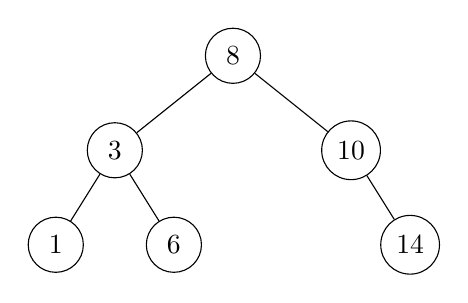
\begin{tikzpicture}[level distance=1.2cm,
  level 1/.style={sibling distance=3cm},
  level 2/.style={sibling distance=1.5cm},
  every node/.style={circle, draw, minimum size=7mm}]
  \node {8}
    child { node {3}
      child { node {1} }
      child { node {6} } }
    child { node {10}
      child[missing]
      child { node {14} } };
\end{tikzpicture}

\begin{tikzpicture}[level/.style={sibling distance=40mm/#1}, level 3/.style={level distance=7mm}]
  \node[draw] (r) {root}
    child { node[draw] {a} child child { node {c} child { node {d} } child { coordinate (x) } } }
    child { coordinate }
    child { node (n) [red] {b} };
  \draw[dashed] (x) -- (n) (r-1) -- (r-2);
\end{tikzpicture}
\end{document}
